\subsubsection{基于TF-IDF的加权词包}
简单地计算词汇的频数不见得是最好的特征提取方式,尽管我们已经去除了停用词,但是文本中仍然会存在有些词比其他词更重要。
词的重要性随着它在文本中出现的次数成正比增加,但同时又随着它在语料库中出现的频率成反比下降。\\
使用TF-IDF作为词重要性的考核标准是因为:如果一个词在一段文本中出现的频率TF高,并且在其他文本中很少出现,那么我们就认为这个词具有很好的类别区分能力,适合用来分类。\\
词频(term frequency, TF)是指某个词在文本中出现的频率。
对文本$ j $里的词$ t_i $来说,其TF计算方式如下\ref{tf}:
\begin{equation}\label{tf}
  TF_{i, j} = \frac{n_{i, j}}{\sum_{k}n_{k, j}}
\end{equation}
其中$ n_{i, j}$是该词在文本 $ d_j $中出现的次数,而分母则是在文本$ d_j $中所有词出现的次数和。\\
逆向文件频率(inverse document frequency, IDF)是对一个词普遍重要性的度量。
某一个词的IDF,可以由总文本数目除以包含该词的文件的数目,再将得到的商去对数可得。
IDF的计算方式如下\ref{idf}:
\begin{equation}\label{idf}
  IDF_i = \log\frac{{| D |}}{| \{ j: t_i \in d_j \} | + 1}
\end{equation}
其中$ | D | $ 是语料库中的文本总数,$ | \{ j : t_i \in d_j \} | $是包含词 $ t_i $文本数目。\\
由TF和IDF可得TF-IDF的计算方法\ref{tfidf}:
\begin{equation}\label{tfidf}
  TFIDF_{i, j} = TF_{i, j} * IDF_{i}
\end{equation}
某个词在某一文本中的高词语频率,以及该词在这个文本集合中的低文本频率,可以产生出高权重的TF-IDF。
因此,TF-IDF倾向于过滤掉常见的词语,保留重要的词语。\\
我们使用scikit-learn提供的TfidfVectorizer模块(sklearn.feature\_extraction.text.TfidfVectorizer)来计算词汇的TF-IDF值,得到和CountVectorizer计算结果一样大小的矩阵,然后将这两个矩阵按元素相乘,得到词包的TF-IDF加权特征。
以这个特征集合来训练分类器,得到如下图\ref{fig:3croctfidf}所示的ROC曲线。
\begin{figure}[h]
\centering
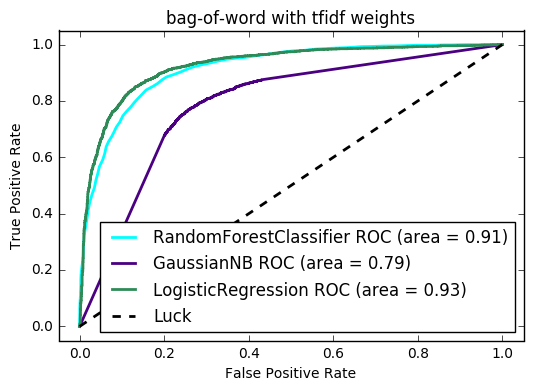
\includegraphics[width=0.9\linewidth]{3c_roc_tfidf}
\caption[roctfidf]{三种模型用TF-IDF加权词包的ROC曲线}
\label{fig:3croctfidf}
\end{figure}

从图中可以看出,这个结果和图4的简单词包的ROC曲线在误差范围内差异不大,但是高斯朴素贝叶斯模型的AUC值却有明显差距。
对于这个差异,我也不是很理解,留待进一步的研究。\\